%%%  Ukázkový text a dokumentace stylu pro text závěrečné (bakalářské a
%%%  diplomové) práce na KI PřF UP v Olomouci
%%%  Copyright (C) 2012 Martin Rotter, <rotter.martinos@gmail.com>
%%%  Copyright (C) 2014 Jan Outrata, <jan.outrata@upol.cz>


%%  Pro získání PDF souboru dokumentu je třeba tento zdrojový text v
%%  LaTeXu přeložit (dvakrát) programem pdfLaTeX.

%%  V případě použití programu BibLaTeX pro tvorbu seznamu literatury
%%  je poté ještě třeba spustit program Biber s parametrem jméno
%%  souboru zdrojového textu bez přípony a následně opět (dvakrát)
%%  přeložit zdrojový text programem pdfLaTeX.

%%  Postup získání Postscriptového souboru je popsán v dokumentaci.


%%  Třída dokumentu implementující styl pro závěrečnou práci. Vybrané
%%  nepovinné parametry (ostatní v dokumentaci):

%%  'master' pro sazbu diplomové práce, jinak se sází bakalářská práce

%%  'field=kód' pro Váš studijní obor, kódy pro diplomovou práci 'uvt'
%%  pro Učitelství výpočetní techniky pro střední školy a 'binf' pro
%%  Bioinformatiku, jinak je výchozí Informatika, a pro bakalářskou
%%  práci 'ainfk' pro Aplikovanou informatiku v kombinované formě,
%%  'inf' pro Informatiku, 'infv' pro Informatiku pro vzdělávání a
%%  'binf' pro Bioinfomatiku, jinak je výchozí Aplikovaná informatika
%%  v prezenční formě

%%  'printversion' pro sazbu verze pro tisk (nebarevné logo a odkazy,
%%  odkazy s uvedením adresy za odkazem, ne odkazy do rejstříku),
%%  jinak verze pro prohlížeč

%%  'biblatex' pro zapnutí podpory pro sazbu bibliografie pomocí
%%  BibLaTeXu, jinak je výchozí sazba v prostředí thebibliography

%%  'language=jazyk' pro jazyk práce, jazyky english pro anglický,
%%  slovak pro slovenský, jinak je výchozí czech pro český

%%  'font=sans' pro bezpatkový font (Iwona Light), jinak výchozí
%%  patkový (Latin Modern)

\documentclass[
%  master,
%  field=inf,
%  printversion,
  biblatex,
%  language=czech,
%  font=sans,
  glossaries,
  index
]{kidiplom}

%% Informace pro úvodní strany. V jazyku práce (pokud není v komentáři
%% uvedeno česky) a anglicky. Uveďte všechny, u kterých není v
%% komentáři uvedeno, že jsou volitelné. Při neuvedení se použijí
%% výchozí texty. Text pro jiný než nastavený jazyk práce (nepovinným
%% parametrem language makra \documentclass, výchozí český) se zadává
%% použitím makra s uvedením jazyka jako nepovinného parametru.

%% Název práce, česky a anglicky. Měl by se vysázet na jeden řádek.
\title{Mobilní aplikace pro pracovníky pečovatelské služby}
\title[english]{Mobile application for workers of the day care}

%% Volitelný podnázev práce, česky a anglicky. Měl by se vysázet na
%% jeden řádek. Výchozí je prázdný.
%% \subtitle{Ukázkový asda text a dokumentace stylu v \LaTeX{}u}
%% \subtitle[english]{Sample text and documentation of the \LaTeX{} style}

%% Jméno autora práce. Makro nemá nepovinný parametr pro uvedení
%% jazyka.
\author{Petr Janiš}

%% Jméno vedoucího práce (včetně titulů). Makro nemá nepovinný
%% parametr pro uvedení jazyka.
\supervisor{Mgr. Janoštík Radek}

%% Volitelný rok odevzdání práce. Výchozí je aktuální (kalendářní)
%% rok. Makro nemá nepovinný parametr pro uvedení jazyka.
\yearofsubmit{2020}

%% Anotace práce, včetně anglické (obvykle překlad z jazyka
%% práce). Jeden odstavec!
\annotation{Ukázkový text závěrečné práce na Katedře informatiky
  Přírodovědecké fakulty Univerzity Palackého v Olomouci, který je
  zároveň dokumentací stylu pro text práce v \LaTeX{}u. Zdrojový text
  v \LaTeX{}u je doporučeno použít jako šablonu pro text skutečné
  závěrečné práce studenta.}

\annotation[english]{Sample text of thesis at the \kitextdepten,
  \kitextfacultyen, \kitextuniven{} and, at the same time,
  documentation of the \LaTeX{} style for the text. The source text in
  \LaTeX{} is recommended to be used as a template for real student's
  thesis text.}

%% Klíčová slova práce, včetně anglických. Oddělená (obvykle) středníkem.
\keywords{styl textu; závěrečná práce; dokumentace; ukázkový text}
\keywords[english]{text style; thesis; documentation; sample text}

%% Volitelná specifikace příloh textu práce, i anglicky. Výchozí je '1
%% CD/DVD'.
%\supplements{jedno kulaté placaté CD/DVD s malou kulatou dírou uprostřed}
%\supplements[english]{one round flat CD/DVD with a small round hole in the middle}

%% Volitelné poděkování. Stručné! Výchozí je prázdné. Makro nemá
%% nepovinný parametr pro uvedení jazyka.
\thanks{Thanks}

%% Cesta k souboru s bibliografií pro její sazbu pomocí BibLaTeXu
%% (zvolenou nepovinným parametrem biblatex makra
%% \documentclass). Použijte pouze při této sazbě, ne při (výchozí)
%% sazbě v prostředí thebibliography.
\bibliography{bibliografie.bib}

%% Další dodatečné styly (balíky) potřebné pro sazbu vlastního textu
%% práce.
\usepackage{lipsum}
\usepackage{float}

\begin{document}
%% Sazba úvodních stran -- titulní, s bibliografickými údaji, s
%% anotací a klíčovými slovy, s poděkováním a prohlášením, s obsahem a
%% se seznamy obrázků, tabulek, vět a zdrojových kódů (pokud jejich
%% sazba není vypnutá).
\maketitle

\section{Úvod}
\begin{figure}[hbt]
  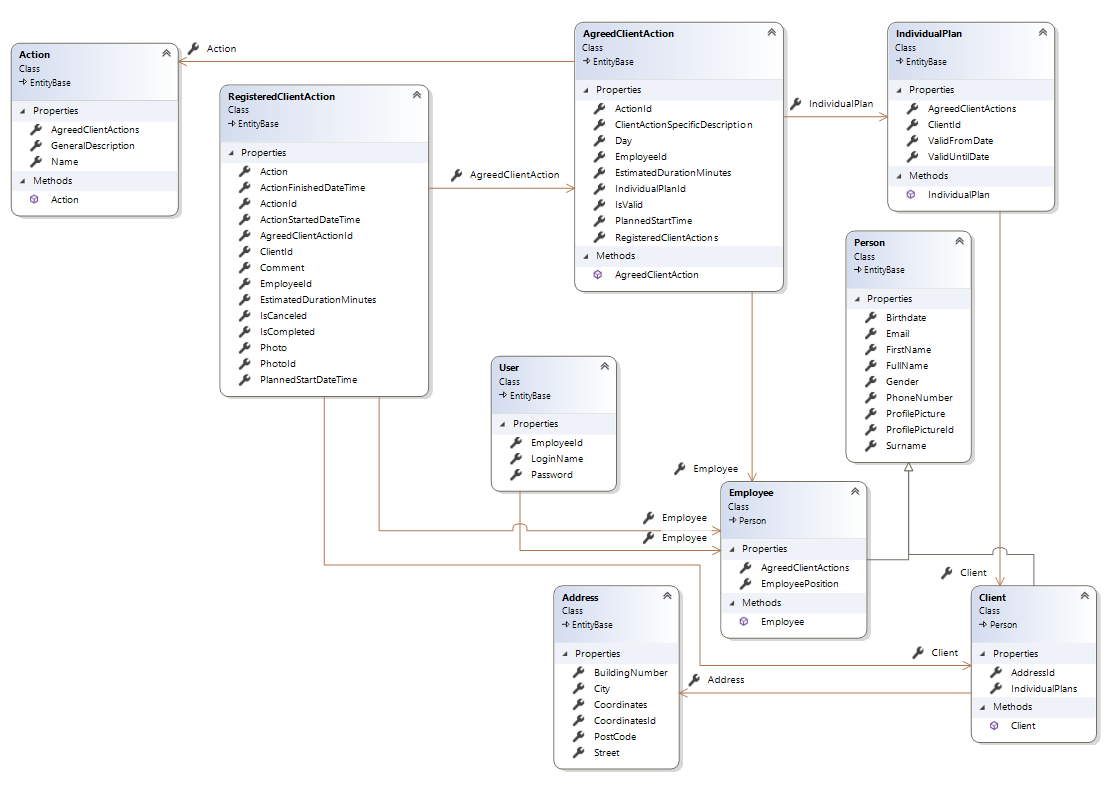
\includegraphics[width=14cm,height=20cm,keepaspectratio]{datovy_model}
  \caption{Datový model}
\end{figure}
\newpage

\section{Vývoj mobilních aplikací}
Mobilní aplikace by uživateli měla co nejjednodušeji a nejrychleji umožnit dosáhnout jeho cíle. Tento fakt je potřeba mít na paměti v průběhu celého procesu vývoje. Proto je důležité, aby aplikace běžela plynule a měla jednoduché uživatelské rozhraní. U aplikací určených pro širokou veřejnost, je dobrý návrh a provedení UI, faktorem rozhodujícím o její úspěšnosti na trhu. Co se týče mobilního softwaru vyvíjeného za účelem korporátního použití je to otázka financí pro firmu, která se ho rozhodne používat. Jednodušší ovládaní znamená měně potřebného času a prostředků vynaložených na zaškolení zaměstnanců.

Pro plynulý běh aplikace je důležité hned na začátku vývoje přesně určit za jakými účely bude používána. Tato specifikace společně s platformou na kterou by měl být vývoj cílen jsou rozhodujícími kriterii při výběru frameworku a způsobu vývoje.

V dnešní době se na trhu s mobilními telefony vyskytují v převážné míře pouze dva operační systémy. Android, který podporuje zařízení od vícero výrobců. A iOS od firmy Apple, který je určen přímo pro hardware od toho výrobce. Ovšem tyto systémy mají spoustu rozdílných verzí, samotná zařízení mají rozdílné velikosti, funkce a vnitřní komponenty. Tohle je pravě to, co činí vývoj mobilních aplikací složitým a zdůrazňuje důležitost výběru správné metody. Aby bylo možné toto klíčové rozhodnutí udělat správně je potřeba se seznámit s detaily různých stylů vývoje a frameworky.

\subsection{Nativní vývoj}
Standardní styl vývoje, který byl dříve i jediným možným způsobem. Při této metodě je aplikace tvořena odděleně pro každou platformu zvlášť. Stejný kód je tedy potřeba napsat dvakrát v různých programovacích jazycích a použít různá vývojová prostředí a nástroje. Nehledě na to, že Apple neumožňuje vývoj nativních aplikací na jiném operačním systému než MacOS. 

Pokud by tedy výsledný software měl běžet na obou platformách, což je ve většině případů předpokladem. Firma by musela mít dva týmy, každý pro jednu část a poskytnout rozdílné vybavení. Nejenom, že tímto způsobem bude vývoj trvat dlouho, ale zároveň bude i drahý. Na druhou stranu výsledkem bude snadno udržovatelná a výkonná aplikace umožňující využívat všech funkcí zařízení. Knihovny, které jsou použity spravují samotní vlastníci OS. Je tedy možné rychle nebo úplně bez zásahu reagovat na nové verze systémů a změny v designu nativních komponent. 

Výsledný produkt je potřeba šířit mezi uživatele. K tomuto účelu slouží takzvaný ''Store'' a každá platforma má svůj vlastní. Obě firmy se snaží vytvořit bezpečné prostředí pro uživatele a kontrolují aplikace sdílené pomocí této služby. Otevřená povaha Androidu ovšem umožňuje mít více než jedno centrální místo pro získání aplikace a proto se snaží řešit část bezpečnostních rizik už na straně kódu a knihoven. Apple je v tomto ohledu daleko přísnější a kontroluje každou aplikaci, která je do App Storu přidána. Někdy trvá i několik dní než prohlásí aplikaci nebo aktualizaci za důvěryhodnou. V tomto procesu se kontroluje hlavně jestli produkt opravdu dělá to co vydavatel tvrdí v popisu a splňuje všechny bezpečnostní normy. Tyto bezpečností aspekty za vývojáře do určité míry schopno pohlídat nativní vývojové prostředí a kompilátor. Tímto způsobem je tedy možné se vyhnout neschválení aplikace firmou Apple a bezpečnostních nedostatků na jiných platformách.

Tento přístup je tedy vhodný pro specifické typy projektů:
\begin{itemize}
	\item Tam kde není potřeba, aby výsledná aplikace běžela na obou platformách.
  	\item Je kladen důraz na výkon aplikace, nebo je to z podstaty požadavků nutnost.
  	\item Hraje velkou roli bezpečnost a není žádoucí používaní knihoven a frameworků třetích stran. 
  	\item Neklade se důraz na rychlost vydaní aplikace na trh a cenu produktu.
 \end{itemize}

\subsubsection{Android}
Aplikace pro Android mohou být napsány pomocí jazyků Kotlin, Java a C++. Nástroj Android SDK zkompiluje kód společně s daty a soubory obsahujícími zdrojové kódy do APK, což je archivní soubor s příponou .apk. APK soubor obsahuje všechny komponenty aplikace a zároveň je to soubor, který zařízení s operačním systémem Android používají k instalaci.
\cite{1}
\textit{(volný překlad)}

K vývoji pro platformu Android je tedy potřeba Android SDK a vhodné vývojové prostředí. Dle dokumentace je doporučovaným vývojovým prostředím Android studio. Velkou výhodou je, že tyto nástroje mohou běžet na jakémkoliv operačním systému.

\subsubsection{iOS}
iOS SDK je balíček nástrojů umožňujících vývoj mobilních aplikací na operační systém iOS. Nástroje umožňují vývojáři přistupovat k různým funkcím a službám iOS zařízení jako jsou hardwarové a softwarové atributy. Obsahuje také iPhone simulátory, které kopírují vzhled a pocit z užívání skutečných zařízení. Aby bylo možné aplikaci testovat a distribuovat ji přes App Store je potřeba zaplatit vývojářskou licenci. SDK společně s vývojovým prostředím Xcode pomáhá psát aplikace pro platformu iOS za použití oficialně podporovaných  jazyků, kterými jsou Swift a Objective-C. 
\cite{2}
\textit{(volný překlad)}

\subsection{Multiplatformní vývoj}
Umožňuje vývoj na obě platformy současně a v některých případech pro ně používá i identický kód. Každý framework toto umožňuje trochu jiným způsobem. Základní myšlenka je ale taková, že na rozdíl od nativních aplikací, které komunikují přímo s operačním systémem a zařízením je u multiplatformních aplikací přidána abstraktní mezivrstva neboli nativní obálka. Mezivrstva zaručuje to, že se aplikace pro systém telefonu tváří jako nativní a zároveň umožňuje kódu přístup ke všem periferiím zařízení jako jsou kamera, určovaní polohy, gyroskop atd. Vzhled takto napsaných aplikací bude naprosto totožný s nativní verzí. Tato obálka ovšem zpomaluje chod aplikace, protože každý proces, který vyžaduje komunikaci se systémem přes ní musí projít a mezivrstva jej musí zpracovat. Toto zpomalení je možno považovat za zanedbatelné pokud není cílem vývoje například hra, aplikace s robustním uživatelským rozhraním nebo s velkým množství rychle vstupujících a ?vystupujících? dat. Celkově tato metoda v porovnaní s klasickým přístupem poskytuje levnější a většinou i rychlejší cestu k vývoji aplikace. 

Na druhou stranu projekt může být vystaven riziku zastavení podpory pro zvolený framework, vrstva navíc znamená prostor pro více bezpečnostních nedostatků a každý vývojář musí být obeznámen s detaily fungování obou platforem. I přesto, že je tímto způsobem možné vyvíjet aplikaci na obě platformy za použití počítače s jakýmkoliv operační systémem, tak pro kompilaci a testování kódu bude v případě iOS nutné použít stroj s macOS. 


\subsubsection{React Native}
React Native je open-source framework, který umožňuje vývoj aplikací pro Android a iOS za použití Reactu a nativních možností platformy. Používá skriptovací jazyk JavaScript za pomocí kterého se přistupuje k API konkretní platformy, zároveň popisuje vzhled a chování  uživatelského rozhraní za použití komponent Reactu.
\cite{3}
\textit{(volný překlad)}

Důležitou vlastností je to, že výsledný kód je kompilován do nativního jazyku používaný platformou. Velkou výhodou je, že pokud žádná z poskytovaných knihoven neobsahuje danou funkcionalitu je možné vytvořit modul v některém z nativních jazyků a zaintegrovat jej do projektu. Za kvalitu framewoku mluví to, že je aktuálně nejpoužívanější ve své kategorii a jsou pomoci něj vytvořeny aplikace jako Facebook a Instagram, které denně používají miliony uživatelů.

\subsubsection{Xamarin}
Xamarin je opět platforma, která umožňuje multiplatformní vývoj tentokrát ale s rozdílem, že společně s mobilními verzí je možné tvořit i aplikaci pro Windows. Patří do rodiny nástrojů .NET čili kód je psán v programovacích jazycích C\# a F\#. Microsoft využívá už nabitých zkušeností vývojářů s jejich předešlým nástrojem WPF a architekturou Model-View-ViewModel. Většina kódu je sdílená, Microsoft uvádí až 90\% \cite{4}, ale je možné určité části vytvořit speciálně pro jednu platformu. V této části je struktura kódu a volaní systémového API velice podobná nativnímu vývoji, pouze za použití jiného jazyka. ?MONO?

\subsubsection{Capacitor}
Nástroj, který umožňuje spuštění webových aplikací jako nativní. Takto vytvořené aplikace jsou také nazývaný jako hybridní. Na rozdíl od React Native se kód tvořený HTML, CSS a JavaScriptem nepřekládá. Namísto toho se uvnitř přidané abstraktní vrstvy otevírá takzvané web view. Web view je v podstatě vestavěný webový prohlížeč, který se stará o běh a zobrazení kódu, lze vidět na Obrázku2 !reference!.  

\begin{figure}[H]
  	\centering
 	 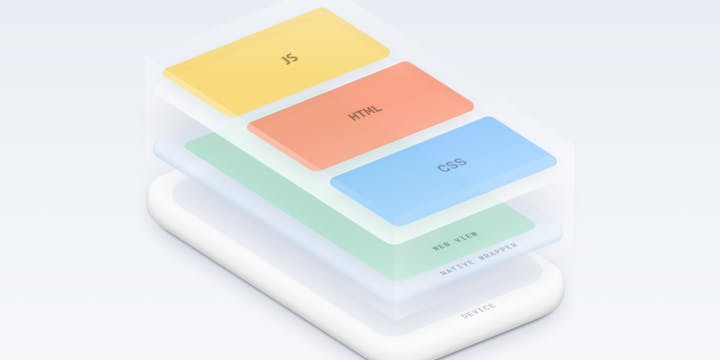
\includegraphics[width=12cm,height=10cm,keepaspectratio]{hybridni_aplikace}
 	 \caption{\cite{5} Architektura hybridních aplikací}
 	 \label{fig:blah}
\end{figure}



Přístup k nativní API je poté zařízen přes pluginy volané z JavaScriptu, které propojují web view s nativní obálkou. Zde už je zpomalení poněkud výraznější a proto se tento způsob doporučuje pouze pro menší až středně velké projekty s nepříliš složitým uživatelským rozhraním, které by potencionálně mohlo na pozadí generovat veliké množství DOM elementů. Možnost z kterékoliv webové aplikace vytvořit nativní aplikaci je hlavní výhodou, ale tvoří problém s nekonzistentním designem uživatelského rozhraní a nepřipraveností webu pro běh na mobilním zařízení. Z tohoto důvodu je dobré používat tento nástroj v kombinaci s některým z framewoků, které jsou k tomu uzpůsobeny.

\subsection{Progresivní webové aplikace(PWA)}
Jsou webové aplikace plně využívající možností moderních webových prohlížečů. Posouvají tím možnosti jejich funkcionality a pocitu z užívaní na úroveň blížící se nativním a multiplatformním aplikacím. Mohou být ale řazeny mezi ostatní mobilní aplikace? Pokud jako definující vlastnosti mobilních aplikací označíme přístup k periferiím zařízení a systémové API, spuštění i bez přístupu k internetu a nutnosti zapnutí webového prohlížeče, provádění procesů na pozadí, potom ano.

Prvním stavebním blokem této technologie jsou takzvané service workery. Service worker je skript, který běží na pozadí odděleně od webové stránky a umožňuje tak funkcionalitu, která nepotřebuje webovou stránku nebo interakci uživatele. \cite{6} \textit{(volný překlad)} Řeší tedy procesy na pozadí a zároveň ukládají kód stažený z webového serveru do aplikační cache a tím umožňují spustit aplikaci bez přístupu k internetu. Na zařízeních používající iOS jsou některé možnosti těchto skriptů omezeny, ale nejedná se o klíčovou funkcionalitu.

Druhou důležitou součástí jsou webové aplikační manifesty. Je to soubor ve formátu JSON, který určuje jak se bude aplikace chovat a vypadat po ''instalaci'' na zařízení. \cite{7} \textit{(volný překlad)} Instalací se v tomto ohledu myslí přidáním ikony na domovskou stránku zařízení. Po spuštění přes tuto ikonu se sice spustí výchozí webový prohlížeč a v něm teprve stránka, ale o tomto procesu uživatel vůbec neví. Prohlížeč totiž nemá žádný ze svých běžných nástrojových lišt a aplikace je otevřena přes celou obrazovku zařízení.

Přístup k periferiím zařízení je potom zařízen různou kombinací možností prohlížeče, HTML5 a JS. Zde je ovšem oproti nativním a multiplatformním aplikacím výběr omezenější.

\subsection{Backend pro mobilní aplikace}
Většina aplikací se neobejde bez serverové části. Buďto z důvodu získání dat nebo komunikace s jinými instancemi aplikace. Server by měl vykonávat většinu výpočetních operací a posílat pouze nezbytně nutná data, aby méně zatěžoval mobilní zařízení. Jako nejlepší postup se tedy může zdát vytvoření vlastní API přímo na míru konkrétní aplikace. Toto řešení zvyšuje výdaje za vývoj i údržbu systému. Zbytečným se stává obzvláště v situacích, kdy by měl server provádět pouze jednoduché operace jako ověření identity uživatele. Pro projekty této povahy je tedy vhodnější vytvářet aplikace bez nutnosti vlastního serveru za pomoci cloudových služeb. Tyto služby umožňují vytvoření databázové struktury a na tomto základě vystavení REST API, které může aplikace konzumovat.
\newpage

\section{Výběr technologií}
Ještě před výběrem konkretních technologií a programovacích jazyků jsem se zamýšlel nad způsobem jak výsledný produkt předat potencionálnímu zákazníkovi. Rozhodnutí nakonec bylo tento problém kompletně eliminovat a celý systém konteinerizovat pomocí nástroje Docker. Kromě výsledných nativních aplikací u kterých to postrádá smysl. Při výběru technologií jsem takto nebyl vázán na prostředí ve kterém systém poběží.

% mozna napsat vse jako swagger/codegen a EF core, MSUNIT
\subsection{Docker}
%% mozna preorganizovat uvod
 
\subsection{Klientské části}
Základním a nejdůležitějším cílem bylo vytvořit aplikaci, která bude funkční na mobilních zařízeních s operačními systémy Android i iOS a zároveň ve webových prohlížečích. Protože jsem byl na vývoj sám a chtěl jsem vytvořit kvalitní aplikaci, nativní vývoj pro každou platformu s následným vytvořením webové verze nepřipadalo v úvahu. Webová aplikace s následným zabalením do nativní obálky je v dané situaci nejvíce vyhovujícím řešením. Jako nástroj pro převod jsem použil výše zmíněny Capacitor. 

Posledním krokem bylo zvolit správný přístup k vývoji webové aplikace. Tradiční způsob tvoření webové stránky za použití HTML, CSS a JavaScriptu by bylo zdlouhavé a potencionálně nebezpečné. Aplikace by očividně obsahovala spoustu kódu v čistém JS, který nemá žádnou kontrolu datových typu, což ve větších projektech může způsobovat chyby, které není lehké odhalit. Další problém by nastal se samotným uživatelským rozhraním. Veškeré UI komponenty by museli být vytvořeny ručně a nebyla by zaručena konzistence se zásadami stylů platformy. Upravovat styl stránky pomocí CSS, tak aby fungovala na zařízeních všech velikostí je sice možné, ale zbytečně náročné. Z těchto důvodů jsem se rozhodl pro použití framework Angular a platformu Ionic, která je navíc výborně kompatibilní s pluginy Capacitoru.

\subsubsection{Angular}
Angular je platforma a framework pro vývoj jednostránkových klientských aplikací za použití HTML a TypeScriptu. Samotný Angular je napsaný v TypeScriptu. Implementuje základní a volitelné funkce jako množinu TypeScriptových knihoven, které je možné importovat do aplikací. \cite{8} \textit{(volný překlad)} 

Jednostránkové klientské aplikace fungují tak, že při prvním přístupu na stránku se ke klientovi stáhnou všechny soubory potřebné k běhu aplikace. Při jakékoliv akci uživatele se stránkou už se nikdy nepřistupuje na webový server. Tento mechanizmus značně ulehčuje service workeru práci s cachovaním a následným spouštěním aplikace v offline režimu, v případě, že by bylo potřeba z aplikace vytvořit PWA.

TypeScript je nadmnožina skriptovacího jazyku JavaScript a přidává do něj možnost typování proměnných, parametrů a návratových hodnot funkcí. Je to objektově orientovaný jazyk podporující funkcionální paradigma s prvky asynchroního programování. Webové prohlížeče ovšem tomuto jazyku nerozumí a proto je potřeba provést proces zvaný transpilace, při kterém se všechny soubory projektu přeloží do souborů s příponou .js, které se navzájem referencují a index.html souboru, který je kořenem tohoto stromu závislostí.

Základními stavebními bloky jsou komponenty a služby. Komponenty se skládají z náhledů a kódu na pozadí. Náhled je HTML kód doplněný o takzvané directivy, které umožňují například psát cykly a podmínky jako atributy HTML tagů. Kód na pozadí je vždy třída, obsahující metody a atributy, které je možné referencovat v náhledu. Služby obsahují funkcionalitu, která přímo nesouvisí s náhledy a je možné je do komponent ''injectovat'' jako závislosti. \cite{8} Framework tedy automaticky nabízí podporu návrhového vzoru Dependecy injection a všechny služby jsou typu Singleton. Architektura založená na používaní komponent velice jednoduše umožňuje znovu použitelnost kódu.

\subsubsection{Ionic}
Platforma, která ulehčuje vývoj webových aplikací cílených na mobilní zařízení. Poskytuje vývojářům množství komponent, které se vzhledově přizpůsobují dle platformy na které běží. Projekty vytvořené pomocí nástrojů, které platforma nabízí jsou plně responzivní. Ionic rozšiřuje základní knihovnu Angularu o nové stavy životních cyklů komponent a navigační strategii, která umožňuje uchovávat si navigační zásobník instancí naposledy otevřených náhledů. Dohromady je díky nim možné implementovat chování navigačních tabů na které jsou uživatelé nativních aplikací zvyklí. 

\subsection{Server}
Chtěl jsem mít plnou kontrolu nad tím jak serverová část zpracovává data a v jakém formátu je posílá na klienta. Vzhledem k zvolené technologii pro aplikaci bylo lepší co nejvíce zodpovědnosti za operace s daty předat serveru a odlehčit tak zařízením na kterých poběží. Proto jsem se rozhodl psát kód serveru sám a přímo na míru místo použití cloudových řešení jako Firebase. 

Základem Angularu zvoleného pro tvorbu klientských částí je JavaScript. JS umí automaticky vytvářet objekty a kolekce z JSON souborů. Angular má navíc v základní knihovně velice dobře zpracovanou podporu pro vytváření HTTP požadavků. Jasnou volbou tedy bylo REST API, které funguje na základě protokolu HTTP a standardním formátem pro přenos dat je právě JSON. S přihlédnutí na budoucí rozšíření bylo žádoucí, aby vybraná technologie umožňovala případné rozšířením o gRPC služby založené na protokolu HTTP/2 kvůli plně duplexní komunikaci.

Dalšími faktory při výběru byly: dobrý vestavěný framework pro prací s databází, podpora pro ověřování identity uživatele pomocí JSON web tokenů, podpora nástroje Swagger pro dokumentaci, nezávislost na operačním systému a ideálně i vestavěná podpora pro Docker. Konečným výběrem tedy byl ASP .NET Core.

\subsubsection{.NET Core}
.NET Core je open source framework pro operační systémy Windows, Linux a macOS. Je to multiplatformní nástupce .NET Frameworku. Projekt je primárně vyvíjen firmou Microsoft a vydáván pod MIT Licencí. \cite{9} \textit{(volný překlad)} Při práci s .NET Corem jsou používány jazyky C\#, F\# a VisualBasic.

ASP .NET Core slouží k vývoji webových aplikací a služeb s tímto vývojem spojených.
\newpage
\section{Server}
%% uvod

\subsection{Databázový modul}
Prvním krokem při vývoji serverové části bylo vytvoření modulu pro práci s databází. Stavebním blokem pro tento modul je Entity Framework Core. Zároveň jsem do tohoto modulu přidal nástroj, který generuje testovací data, který je možno explicitně spustit ve formě konzolové aplikace.

\subsubsection{Datové třídy}
 U tvorby tříd odrážejících strukturu datového modelu (ref obr. 1), bylo potřeba zvolit vhodné datové typy, vyřešit jak simulovat relace mezi jednotlivými tabulkami a rozdíl mezi povinnými a nepovinnými parametry:
\begin{itemize}
	\item Název tabulky určuje anotace (ref kod.1) na řádku 1. 
	\item Jako identifikátor jsem zvolil datový typ Guid, který umožňuje přímo identifikovat určitý záznam v databázi.
	\item Atributy s hodnotovými datovými typy jsou označeny jako nullable pokud nejsou povinné.
	\item K atributům s referenčními datovými typy je přidána anotace Required pokud jsou povinné, (ref kod. 1) řádky 4 a 7.
	\item V případě relace 1:N. Jsou relace simulovány kombinací atributu pro uložení cizího klíče a referencí na instanci třídy reprezentující jinou tabulku neboli navigační atribut pro stranu relace 1, (ref kod. 1) řádky 10 a 11. Pro stranu N bude navigační atribut kolekce těchto typů.
\end{itemize}

\begin{kicode}{csharp}{}{Kód reprezentující entitu.}
[Table("User")]
    public class User : EntityBase
    {
        [Required]
        public string LoginName { get; set; }

        [Required]
        public string Password { get; set; }

        public Guid EmployeeId { get; set; }

        public virtual Employee Employee { get; set; }
    }
\end{kicode}

\subsubsection{Db Context}
Datové třídy jsou spojeny ve třídě DbContext jejíž instance reprezentuje spojení s databází. Na úrovni této třídy je zároveň řešeno jaký databázový poskytovatel bude použit. Dle toho je potřeba integrovat správnou knihovnu. Tato integrace je naštěstí triviální a je možné připojení k serverům s jiným poskytovatelem libovolně měnit s minimem úsilí. Právě tato třída umožňuje ostatním modulům číst a zapisovat data do databáze. Zodpovědností modulu přistupujícího k datům je předat contextu connection string, díky kterému je možné spojení navázat. V celém projektu je pro práci s daty použit dotazovací jazyk LINQ s rozšíření, které umožňuje dotazování za pomocí lamba výrazů.

Balíček EFCore Tool umožňuje za použití příkazové řádky vytvářet Migrace. Migrace je automaticky vygenerovaný kód lišící se dle momentálně použitého databázového poskytovatele popisující strukturu databáze danou DbContextem. Tento kód poté může být použit při volaní metody Migrate, která do aktuálně připojené instance databáze vytvoří onu strukturu. Tento přístup se nazývá Code first.

Pro načítaní hodnot do navigačních atributů do objektů představujících záznamy v databázi je použita metoda Lazy loading. Na rozdíl od ostatních možných přístupů zaručuje, že data budou načtena vždy až to opravdu bude nutné a současně o to není potřeba explicitně žádat. Toho efektu jsem docílil označením všech klíčových atributů jako virtuálních, což umožňuje aby se na na jejich místě vytvořili proxy objekty.

\subsection{Struktura API}
%% uvod?
\begin{figure}[H]
  	\centering
 	 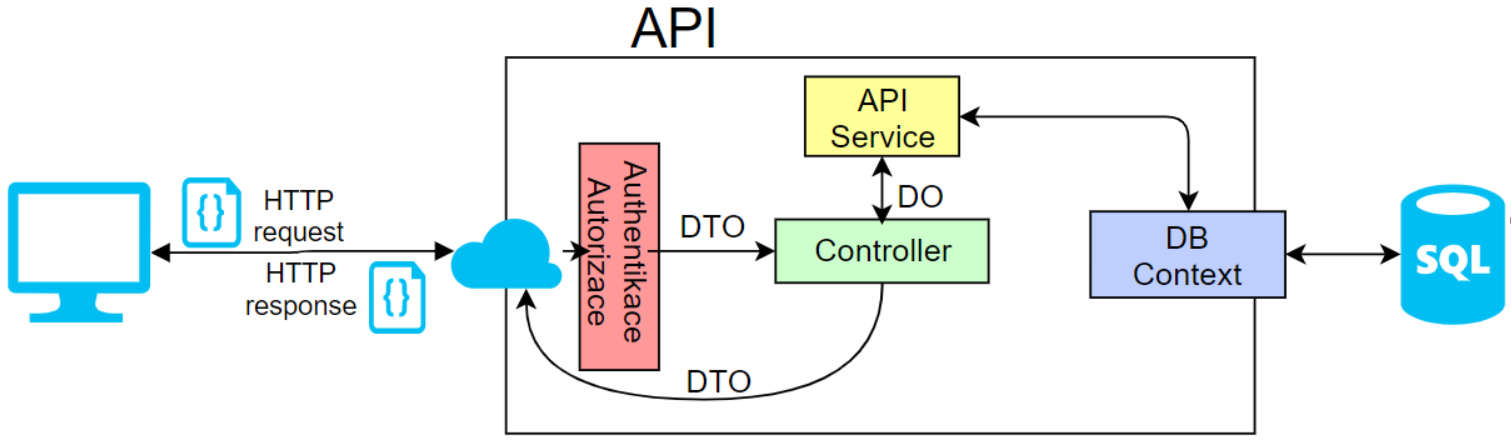
\includegraphics[width=14cm,height=10cm,keepaspectratio]{API_Diagram}
 	 \caption{Diagram struktury API}
\end{figure}

\subsubsection{API controllery}
Pomocí controlleru se definuje celá struktura API. Obsahují metody, které jsou volány pomoci HTTP requestů. 

\begin{kicode}{csharp}{}{Ukázka kódu controlleru}
	[Route("api/[controller]")]
	[ApiController]
	[Authorize]
    public class EmployeeController : DssBaseController
    {
        private readonly IEmployeeApiService _employeeApiService;

        public EmployeeController(IEmployeeApiService employeeApiService)
        {
            _employeeApiService = employeeApiService;
        }

        [HttpPost]
        [Authorize(Roles = "Manager")]
        public EmployeeDetailDTO CreateEmployee(EmployeeDetailDTO dto)
        {
            var employee = MapDetailDtoToEmployee(dto);
            var createdEmployee = _employeeApiService.CreateEmployee(employee);
            var createdDto = MapEmployeeToDetailDto(createdEmployee);

            return createdDto;
        }
        ...
\end{kicode}

Proces životního cyklu z pohledu API začíná ve chvíli, kdy na nějaký z endpointů přijde požadavek. Který controller by ho měl zpracovat záleží na použité směrovací strategii a URI na kterou byl zaslán. S použitím výchozího směrování, jako jsem použil já a definice cesty v anotaci (ref. code 2) řádek 1 by tento controller obsluhoval všechny požadavky na  adrese: \textit{[základní\_adresa]}/employee/... Jestli je potřeba, aby byl požadavek opatřen platným tokenem určuje anotace Authorize. (ref. code 2) řádkem 3 je tedy dáno, že všechny  požadavky, které tímto controllerem budou obslouženy musí být takto zabezpečeny.   

HTTP metod je dohromady 8, ale v projektu jsou použity pouze 4 z nich a při jejich použití jsem se držet konvencí: 
\begin{itemize}
	\item \textbf{GET} - je používána pro získání informací ze serveru. Měla by být používána pouze pro získání dat a neměla by na data mít žádný jiný efekt. \cite{10} \textit{(volný překlad)}
	\item \textbf{POST} - používá se pro zaslání dat na server.\cite{10} \textit{(volný překlad)}
	\item \textbf{PUT} - Nahrazuje všechny aktuální reprezentace daného zdroje nahrávaným  obsahem.\cite{10} \textit{(volný překlad)}
	\item \textbf{DELETE} - Smaže všechny aktuální výskyty zdroje uvedeného v URI.\cite{10} \textit{(volný překlad)}
\end{itemize}
Metoda \textit{CreateEmployee} bude díky anotaci (ref. code 2) na řádku 13 data ukládat a reagovat pouze na POST requesty. 

Posledním aspektem, který je potřeba zmínit je rozdělení rolí. V systému jsou role dvě: pracovník pečovatelské služby a vedoucí pracovník. Každá role má jiná práva a tím pádem může přistupovat k různým endpointům a získávat tak odlišná data. Pracovník pečovatelské služby je základní role s minimálními oprávněními pro vstup do systému, proto metody konzumovány tímto typem účtů není potřeba explicitně kontrolovat. Při přihlášení se do tokenu ukládá informace(claim - viz ref sekce zabezpečení) o této roli a ta je kontrolována, pokud je metoda označena stejně jako (ref. code 2) na řádku 14.

Framework automaticky serializuje a deserializuje objekty z a do formátu JSON. Pro vývojáře je tento proces naprosto transparentní a muže rovnou pracovat s objekty jak jsou definovány v kódu. Z důvodu bezpečnosti, znovupoužitelnosti a možné budoucí rozšiřitelnosti kódu jsem se pro práci s objekty a daty rozhodl použít strategii řídící se následujícími pravidly: 
\begin{itemize}
	\item Návratový typ metody controlleru je vždy DTO obsahující jen ty nejnutnější údaje.
	\item DTO objekty existují pouze v rozsahu controlleru(předchází problému kruhových závislostí).
\end{itemize} 
Lze pozorovat, že metoda (ref. code 2) na řádcích 15-22 se tohoto principu drží. Na (ref. obr.2) je toto demonstrováno mezi conrollerem a API službou mezi kterými se posílají pouze Domain Objects.

\subsubsection{API služby}
Všechny operace s databází jsou striktně prováděny pouze v této skupině tříd. Správnost databázových dotazů je totiž jediným místem, kde může dojít k sémantickým chybám. Tyto třídy proto implementují rozhraní obsahující všechny jejich veřejné metody, což činí případné Mockování v následném testování možným. Navíc díky dodržováni pravidel o DTO mohou být kdykoliv v budoucnu využity znovu v jiném modulu. 

\subsubsection{DI a propagace konfigurace}
Framework má zabudovanou automatickou podporu pro návrhový vzor Dependecy Injection(DI). Toho jsem využil pro distribuci DbContextu do API služeb a tech zase do controlleru. Výsledek procesu je vidět na (ref. code 2) řádcích 6-11. Controller závisí na\textit{EmployeeApiService}, která je reprezentována svým rozhraním a DI kontejner při volání tohoto konstruktoru automaticky poskytne její instanci jako parametr.

ASP .NET Core má komplexní systém možností konfigurace, která zvládne konzumovat konfiguraci z mnoha různých zdrojů najednou, upřednostnit parametry s větší prioritou a následně je sloučit. Tohoto je využito například při nastavování proměnných prostředí při spouštění Docker kontejneru.

\subsubsection{Zabezpečení}
Všechny požadavky musí v hlavičce obsahovat platný token, jinak je API odmítne obsloužit. Tyto Json Web Tokeny vystavuje jediný nezabezpečený endpoint, který přímá jako parametry jméno a heslo uživatele. Hesla jsou v databázi uložena v hashované podobě, proto je nutno udělat to stejné a převést heslo pomocí hashovací funkce MD5. Pokud ověření proběhne v pořádku je vytvořen nový token, který je podepsán soukromým klíčem a jsou do něj zakódovány informace jako jméno uživatele, kdo je konzument a vydavatel tokenu a role. Tyto informace se nazývají claimy a je možné je z tokenu pomocí určitých nástrojů vyčíst. Jediná informace, která zaručuje bezpečnost je právě soukromý klíč. 

\subsubsection{Swagger a automatická dokumentace}
Pro účely dokumentace API jsem použil nástroj Swagger, který automaticky zpracuje její strukturu a poskytne jí v podobě uživatelského rozhraní a JSON souboru. V produkci je žádoucí tuto funkci vypnout nebo zabezpečit ověřením identity.

\begin{figure}[H]
  	\centering
 	 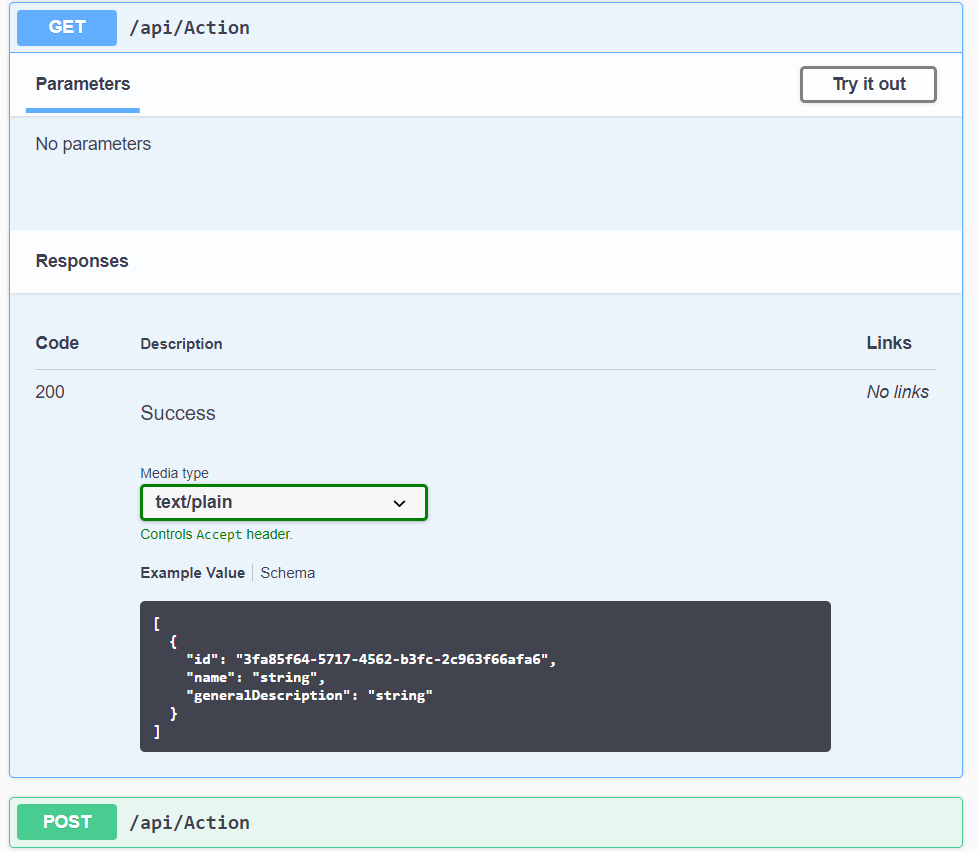
\includegraphics[width=14cm,height=10cm,keepaspectratio]{Swagger_UI}
 	 \caption{Ukázka automatické dokumentace pomocí Swaggeru}
\end{figure}

\subsection{Testování částí}
Testování částí je úroveň testovaní softwaru, kde jsou testovány individuální komponenty nebo části. Smyslem je ověřit, zdali se každá část chová jak byla navržena. Část je nejmenší testovatelná jednotka jakéhokoliv softwaru.\cite{11} \textit{(volný překlad)}

Testování částí jsem v systému použil pro testování metod API služeb, které provádí složitější databázové dotazy a operace nad těmito daty. Všechny tyto metody používají DbContext pro přístup do databáze. Tento přístup bylo potřeba nahradit testovací instancí databáze, která bude bude na začátku každého testu obsahovat prázdnou strukturu tabulek a po jeho skončení přestane existovat. Pro dosažení tohoto efektu byl DbContextu konfigurován pro používání databáze v paměti.

Každý test se skládá z těchto stavů: 
\begin{itemize}
	\item \textbf{Arrange} - připraví strukturu dat, tak aby testovala přesnou funkcionalitu testované části.
	\item \textbf{Act} - spustí kód testované části.
	\item \textbf{Assert} - porovnává vrácené výsledky s očekávanými výsledky, pokud se liší vyvolá chybu.
\end{itemize}

\newpage

\section{Klientské části}
% uvod

\subsection{Multiplatformní aplikace}
%% ?uvod?

\subsubsection{Komunikace se serverem}

%% komunikace s api - swagger, interceptor datumy
%% authentikace/login screen
%% client casche, poloha, vzdalenost, dopocitani chybejici adresy google map api
%% rozvrh - infinit loader, stavy, datepicker, detail, stopky
%% mapa - navigace v google mapach, 
%% clientsky detail, individualni plan
%% uprava pro desktopy


\subsection{Managerská webová aplikace}
%% uvod
%% kalendar a drag and drop

\newpage

\section{Nasazení}

\subsection{Kontejnerizace}

\subsection{Azure}

\subsection{CI/CD}

\newpage


\begin{thebibliography}{9}
 \bibitem{1} https://developer.android.com/guide/components/fundamentals
 \bibitem{2} https://en.wikipedia.org/wiki/IOS_SDK
 \bibitem{3} https://reactnative.dev/docs/intro-react-native-components
 \bibitem{4} https://docs.microsoft.com/en-us/xamarin/get-started/what-is-xamarin
 \bibitem{5} https://ionicframework.com/resources/articles/what-is-hybrid-app-development
 \bibitem{6} https://developers.google.com/web/fundamentals/primers/service-workers#what_is_a_service_worker 
  \bibitem{7} https://web.dev/add-manifest/
  https://angular.io/guide/architecture
  \bibitem{9} https://en.wikipedia.org/wiki/.NET_Core
  \bibitem{10} https://www.tutorialspoint.com/http/http_methods.htm
  \bibitem{11} http://softwaretestingfundamentals.com/unit-testing/
 \end{thebibliography}


\newpage
%% Obsah přiloženého CD/DVD. Poslední příloha. Upravte podle vlastní
%% práce!
\section{Obsah přiloženého CD/DVD} \label{sec:ObsahCD}

Na samotném konci textu práce je uveden stručný popis obsahu
přiloženého CD/DVD, tj.~jeho závazné adresářové struktury, důležitých
souborů apod.

\begin{description}

\item[\texttt{bin/}] \hfill \\
  Instalátor \textsc{Instalator} programu, popř.~program
  \textsc{Program}, spustitelné přímo z~CD/DVD. / Kompletní adresářová
  struktura webové aplikace \textsc{Webovka} (v~ZIP archivu) pro
  zkopírování na webový server. Adresář obsahuje i~všechny runtime
  knihovny a~další soubory potřebné pro bezproblémový běh instalátoru
  a~programu z~CD/DVD / pro bezproblémový provoz webové aplikace na
  webovém serveru.

\item[\texttt{doc/}] \hfill \\
  Text práce ve formátu PDF, vytvořený s~použitím závazného stylu KI
  PřF UP v~Olomouci pro závěrečné práce, včetně všech příloh,
  a~všechny soubory potřebné pro bezproblémové vygenerování PDF
  dokumentu textu (v~ZIP archivu), tj.~zdrojový text textu, vložené
  obrázky, apod.

\item[\texttt{src/}] \hfill \\
  Kompletní zdrojové texty programu \textsc{Program} / webové aplikace
  \textsc{Webovka} se všemi potřebnými (příp.~převzatými) zdrojovými
  texty, knihovnami a~dalšími soubory potřebnými pro bezproblémové
  vytvoření spustitelných verzí programu / adresářové struktury pro
  zkopírování na webový server.

\item[\texttt{readme.txt}] \hfill \\
  Instrukce pro instalaci a~spuštění programu \textsc{Program}, včetně
  všech požadavků pro jeho bezproblémový provoz. / Instrukce pro
  nasazení webové aplikace \textsc{Webovka} na webový server, včetně
  všech požadavků pro její bezproblémový provoz, a~webová adresa, na
  které je aplikace nasazena pro účel testování při tvorbě posudků
  práce a~pro účel obhajoby práce.

\end{description}

Navíc CD/DVD obsahuje:

\begin{description}

\item[\texttt{data/}] \hfill \\
  Ukázková a~testovací data použitá v~práci a~pro potřeby testování
  práce při tvorbě posudků a~obhajoby práce.

\item[\texttt{install/}] \hfill \\
  Instalátory aplikací, runtime knihoven a~jiných souborů potřebných
  pro provoz programu \textsc{Program} / webové aplikace
  \textsc{Webovka}, které nejsou standardní součástí operačního
  systému určeného pro běh programu / provoz webové aplikace.

\item[\texttt{literature/}] \hfill \\
  Vybrané položky bibliografie, příp.~jiná užitečná literatura
  vztahující se k~práci.

\end{description}

U~veškerých cizích převzatých materiálů obsažených na CD/DVD jejich
zahrnutí dovolují podmínky pro jejich šíření nebo přiložený souhlas
držitele copyrightu. Pro všechny použité (a~citované) materiály,
u~kterých toto není splněno a~nejsou tak obsaženy na CD/DVD, je uveden
jejich zdroj (např.~webová adresa) v~bibliografii nebo textu práce
nebo v souboru \texttt{readme.txt}.

%% -------------------------------------------------------------------

%% Sazba volitelného seznamu zkratek, za přílohami.
\printglossary

%% Sazba povinné bibliografie, za přílohami (případně i za seznamem
%% zkratek). Při použití BibLaTeXu použijte makro
%% \printbibliography. jinak prostředí thebibliography. Ne obojí!

%% Sazba i v textu necitovaných zdrojů, při použití
%% BibLaTeXu. Volitelné.
\nocite{*}
%% Vlastní sazba bibliografie při použití BibLaTeXu.
\printbibliography

%% Bibliografie, včetně sazby, při nepoužití BibLaTeXu.
% \begin{thebibliography}{9}
%\bibitem{kniha2} \uppercase{Hawke}, Paul. NanoHttpd: Light-weight HTTP server designed for embedding in other applications. GitHub [online]. 2014-05-12. [cit. 2014-12-06]. Dostupné z: \url{https://github.com/NanoHttpd/nanohttpd}
%
%\bibitem{jeske13} \uppercase{Jeske}, David; \uppercase{Novák}, Josef. Simple HTTP Server in \csharp: Threaded synchronous HTTP Server abstract class, to respond to HTTP requests. CodeProject: For those who code [online]. 2014-05-24. [cit. 2014-12-06]. Dostupné z: \url{http://www.codeproject.com/Articles/137979/Simple-HTTP-Server-in-C}
%
%\bibitem{uzis2012} \uppercase{ÚSTAV ZDRAVOTNICKÝCH INFORMACÍ A STATISTIKY ČR}. Lékaři, zubní lékaři a farmaceuti 2012 [online]. Praha 2, Palackého náměstí 4: Ústav zdravotnických informací a statistiky ČR, 2012 [cit. 2014-12-06]. ISBN 978-80-7472-089-5. Dostupné z: \url{http://www.uzis.cz/publikace/lekari-zubni-lekari-farmaceuti-2012}
% \end{thebibliography}

%% Sazba volitelného rejstříku, za bibliografií.
\printindex

\end{document}
